
%----------------------------------------------------------
%	PACKAGES AND OTHER DOCUMENT CONFIGURATIONS
%----------------------------------------------------------

\documentclass[
11pt, % The default document font size, options: 10pt, 11pt, 12pt
oneside, % Two side (alternating margins) for binding by default, uncomment to switch to one side
english, % ngerman for German
singlespacing, % Single line spacing, alternatives: onehalfspacing or doublespacing
%draft, % Uncomment to enable draft mode (no pictures, no links, overfull hboxes indicated)
%nolistspacing, % If the document is onehalfspacing or doublespacing, uncomment this to set spacing in lists to single
%liststotoc, % Uncomment to add the list of figures/tables/etc to the table of contents
toctotoc, % Uncomment to add the main table of contents to the table of contents
%parskip, % Uncomment to add space between paragraphs
%nohyperref, % Uncomment to not load the hyperref package
headsepline, % Uncomment to get a line under the header
%chapterinoneline, % Uncomment to place the chapter title next to the number on one line
%consistentlayout, % Uncomment to change the layout of the declaration, abstract and acknowledgements pages to match the default layout
]{MastersDoctoralThesis} % The class file specifying the document structure

\ProvidesClass{ieeeconf}[2004/1/15 revision V1.6b by Pradeep Misra]

\usepackage[utf8]{inputenc} % Required for inputting international characters
\usepackage[T1]{fontenc} % Output font encoding for international characters

\usepackage{mathpazo} % Use the Palatino font by default

%\usepackage[backend=bibtex,style=authoryear,natbib=true]{biblatex} % Use the bibtex backend with the authoryear citation style (which resembles APA)
\usepackage[numbers]{natbib}
%\addbibresource{example.bib} % The filename of the bibliography

\usepackage[autostyle=true]{csquotes} % Required to generate language-dependent quotes in the bibliography

\usepackage{graphicx}
\usepackage{caption}
\usepackage{subcaption}
\usepackage{float}

\usepackage{listings}
\usepackage{color}

\definecolor{dkgreen}{rgb}{0,0.6,0}
\definecolor{gray}{rgb}{0.5,0.5,0.5}
\definecolor{mauve}{rgb}{0.58,0,0.82}

\lstset{frame=tb,
  language=Java,
  aboveskip=3mm,
  belowskip=3mm,
  showstringspaces=false,
  columns=flexible,
  basicstyle={\small\ttfamily},
  numbers=none,
  numberstyle=\tiny\color{gray},
  keywordstyle=\color{blue},
  commentstyle=\color{dkgreen},
  stringstyle=\color{mauve},
  breaklines=true,
  breakatwhitespace=true,
  tabsize=3
}
\usepackage{titlesec}
\titlespacing*{\section}
{0pt}{5.5ex plus 1ex minus .2ex}{4.3ex plus .2ex}
\titlespacing*{\subsection}
{0pt}{5.5ex plus 1ex minus .2ex}{4.3ex plus .2ex}
\titlespacing*{\paragraph}
{0pt}{5.5ex plus 1ex minus .2ex}{4.3ex plus .2ex}
\titlespacing*{\subparagraph}
{0pt}{5.5ex plus 1ex minus .2ex}{4.3ex plus .2ex}
%-----------------------------------------------------------------------------
%	MARGIN SETTINGS
%-----------------------------------------------------------------------------

\geometry{
	paper=a4paper, % Change to letterpaper for US letter
	inner=2.5cm, % Inner margin
	outer=3.8cm, % Outer margin
	bindingoffset=.5cm, % Binding offset
	top=1.5cm, % Top margin
	bottom=1.5cm, % Bottom margin
	%showframe, % Uncomment to show how the type block is set on the page
}

%-----------------------------------------------------------------------------
%	THESIS INFORMATION
%-----------------------------------------------------------------------------

\thesistitle{Refining Index Storage in NoSQL Graph Databases} % Your thesis title, this is used in the title and abstract, print it elsewhere with \ttitle
\title{Refining Index Storage in NoSQL Graph Databases}
\supervisor{Dr. Srikanta J. Bedathur} % Your supervisor's name, this is used in the title page, print it elsewhere with \supname
\examiner{} % Your examiner's name, this is not currently used anywhere in the template, print it elsewhere with \examname
\degree{Bachelor of Technology} % Your degree name, this is used in the title page and abstract, print it elsewhere with \degreename
\author{Mayank Rajoria \\Prakhar Gupta \\Prakhar Agrawal } % Your name, this is used in the title page and abstract, print it elsewhere with \authorname
\addresses{} % Your address, this is not currently used anywhere in the template, print it elsewhere with \addressname

\subject{} % Your subject area, this is not currently used anywhere in the template, print it elsewhere with \subjectname
\keywords{} % Keywords for your thesis, this is not currently used anywhere in the template, print it elsewhere with \keywordnames
\university{\href{http://www.iitd.ac.in}{Indian Institute of Technology, Delhi}} % Your university's name and URL, this is used in the title page and abstract, print it elsewhere with \univname
\department{\href{http://www.cse.iitd.ac.in}{Department of Computer Science and Engineering}} % Your department's name and URL, this is used in the title page and abstract, print it elsewhere with \deptname
 
% \group{\href{http://researchgroup.university.com}{Research Group Name}} % Your research group's name and URL, this is used in the title page, print it elsewhere with \groupname
\faculty{\href{http://bedathur.net}{}} % Your faculty's name and URL, this is used in the title page and abstract, print it elsewhere with \facname

\AtBeginDocument{
\hypersetup{pdftitle=\ttitle} % Set the PDF's title to your title
\hypersetup{pdfauthor=\authorname} % Set the PDF's author to your name
\hypersetup{pdfkeywords=\keywordnames} % Set the PDF's keywords to your keywords
}

\begin{document}

\frontmatter % Use roman page numbering style (i, ii, iii, iv...) for the pre-content pages

\pagestyle{plain} % Default to the plain heading style until the thesis style is called for the body content

%-----------------------------------------------------------------------------
%	TITLE PAGE
%-----------------------------------------------------------------------------

\begin{titlepage}
\begin{center}

\vspace*{.06\textheight}
{\scshape\LARGE \univname\par}\vspace{1.5cm} % University name
\textsc{\Large B.Tech Project Thesis}\\[0.5cm] % Thesis type

\HRule \\[0.4cm] % Horizontal line
{\huge \bfseries \ttitle\par}\vspace{0.4cm} % Thesis title
\HRule \\[1.5cm] % Horizontal line
 
\begin{minipage}[t]{0.4\textwidth}
\begin{flushleft} \large
\emph{Author:}\\
\href{}{\authorname} % Author name - remove the \href bracket to remove the link
\end{flushleft}
\end{minipage}
\begin{minipage}[t]{0.4\textwidth}
\begin{flushright} \large
\emph{Supervisor:} \\
\href{}{\supname} % Supervisor name - remove the \href bracket to remove the link  
\end{flushright}
\end{minipage}\\[3cm]
 
\vfill

\large \textit{A thesis submitted in fulfillment of the requirements\\ for the degree of \degreename}\\[0.3cm] % University requirement text
\textit{in the}\\[0.4cm]
DAIR\\Department of Computer Science and Engineering\\[2cm] % Research group name and department name
 
\vfill

{\large \today}\\[4cm] % Date
%\includegraphics{Logo} % University/department logo - uncomment to place it
 
\vfill
\end{center}
\end{titlepage}


\cleardoublepage


\begin{abstract}

\addchaptertocentry{\abstractname} % Add the abstract to the table of contents
$\:$\\
Graph databases such as Neo4j, JanusGraph/Titan etc. are increasingly becoming popular due to the flexible data model they provide. However, writing optimal queries on these databases using the dataflow query language, Gremlin, remains an interesting problem. In this project, we explore ways to optimize these Gremlin queries by exploiting the flexibility --viz., schema -- of the graph database.\\\\
Specifically, we try to achieve this by storing the index structure as a part of the graph database itself (thus removing dependency on third party application like the elastic search or solr). We explore this approach towards the following four-fold objectives: (a) reduce the moving components from a graph database, (b) remove the application layer overheads in terms of using external applications like solr (c) offer flexibility in terms of index structures one can design and play with and (d) explore other unexplored ways of traversal e.g. traveling through index to data and then going up some other index to get cumulative number etc.

\end{abstract}


%-----------------------------------------------------------------------------
%	LIST OF CONTENTS/FIGURES/TABLES PAGES
%-----------------------------------------------------------------------------

\tableofcontents % Prints the main table of contents

% \listoffigures % Prints the list of figures

% \listoftables % Prints the list of tables

%-----------------------------------------------------------------------------
%	ABBREVIATIONS
%-----------------------------------------------------------------------------

% \begin{abbreviations}{ll} % Include a list of abbreviations (a table of two columns)

% \textbf{LAH} & \textbf{L}ist \textbf{A}bbreviations \textbf{H}ere\\
% \textbf{WSF} & \textbf{W}hat (it) \textbf{S}tands \textbf{F}or\\

% \end{abbreviations}

%-----------------------------------------------------------------------------
%	THESIS CONTENT - CHAPTERS
%-----------------------------------------------------------------------------

\mainmatter % Begin numeric (1,2,3...) page numbering

\pagestyle{thesis} % Return the page headers back to the "thesis" style

% Include the chapters of the thesis as separate files from the Chapters folder
% Uncomment the lines as you write the chapters
\setstretch{1.15}

% Chapter 1

\chapter{Introduction} % Main chapter title

\label{Chapter1} % For referencing the chapter elsewhere, use \ref{Chapter1} 

%----------------------------------------------------------------------------------------

% Define some commands to keep the formatting separated from the content 
\newcommand{\keyword}[1]{\textbf{#1}}
\newcommand{\tabhead}[1]{\textbf{#1}}
\newcommand{\code}[1]{\texttt{#1}}
\newcommand{\file}[1]{\texttt{\bfseries#1}}
\newcommand{\option}[1]{\texttt{\itshape#1}}

%----------------------------------------------------------------------------------------

\section{Motivation}
NoSQL and Graph databases are alternatives to the already existing SQL approaches used in web and cloud applications. They have recently gained a wide spread acceptance, both in industry and academia. This has been due the their ability to handle an increasing scale of operations and the fact that they allow data to be stored in a way it is modeled. \\
\\
These databases do support indexes but require a separate index backend to create and maintain this index. This not only adds more moving components to the database but also hampers the flexibility to use the set of index structures offered by the application alone. This separation of index, from the data, at an application level causes inefficiencies in its usage. This is due to the inter-application overheads involved in the communictaion between the graph database store and the index backend. Hence, exploiting the flexible schema of graph databases, we have devised a way to store the index along with the data, and reduce these additional overheads.

%----------------------------------------------------------------------------------------

\section{Approach}
Schema flexibility in Graph databases allows us to "rewire" a graph in the database by introducing new vertices and edges/relationships between these and original vertices. We create these new, or "ghost" edges and vertices, based on their utility in making the queries faster. These vertices and edges should ideally be invisible to the end-user and play the role of an \textit{index} in these graph databases. \\
\\
These will allow us to perform faster traversal in the graph and hence would speed up the queries we wish to run on the graph. We construct these elements and put them as a layer in the graph database itself, as "ghost" nodes and edges. Clearly, this kind of rewiring is going to bloat up the size of the graph, hence we must chose the vertices and edges to be added carefully. This decision is should be made on the basis of a set of static query workloads given initially. Currently we do not have a metric to base our decision regarding the choice of the index but use intuition for all further experiments stated in the paper.\\
\\
Considering this flexibility of the graph, a natural way to introduce powerful indexing capabilities within the graph is to store the index itself as a layer in the graph. We utilize the fact that most of the traditional indexes can be represented as trees (for eg B-Tree), which are essentially graphs. For instance, it is possible to store a multi-dimensional index structure such as R-Tree simply in the graph database starting from linking vertices which have overlapping bounding boxes, and going on to construct multiple layers of this relationship in the same manner as a traditional R-Tree. \\
\\
Finally, to understand the impact of these methods, we need to run test on a benchmark. We choose the LDBC's  \cite{benchmark} (Linked Data Benchmark Council) Business Intelligence Workload which consists a various complex structured queries for analyzing the behaviour of various parts of a social network. These workloads help us highlight the effect of our methods on the performance. 

\section{Choice of Benchmark}
LDBC (Linked Data Benchmark Council)  \cite{benchmark} is an organization that develops benchmarks that allow various Graph Database management systems to be tested for their capabilities and their performance. We use the Social Network benchmark developed by them. This benchmark has vertices and edges in the structure of a typical social network i.e. users with details about them, people they know, their posts and likes and comments on posts. It also has a set of both interactive and business intelligence queries that operate on this data. Also it has a data generator package which can create social network databases of varied sizes.\\
\\
Social Networks are one of the best examples of applications of Graph databases and therefore they form a great choice for queries which can involve a given number of hops (example a 2 hop from a person would give the people known to the people he knows). The indexes we are creating can thus be tested for efficiency by cutting down on the number of such hops. So social networks are a good choice for benchmarking.\\
\\
LDBC SNB workload has some really good properties that allows us to create synthetic data which closely mimics the data from real social networks. It enforces on the network structure the power law distribution in terms of various properties as well as the short diameters of the graph that are generally common in social networks. It is also generates property values which are realistic in nature and generated from correlated value distributions of these properties. Temporal correlations and presence of flash mobs is also something that makes this a really valuable benchmark for any system that is to work in a real world scenario.\\
\\
For our testing, we only deal with the Business Intelligence queries of the Social Network benchmark. This consists of complex structured query workloads.  Most of these queries require us to find and group vertices that satisfy certain given constraints. Since we are using the Gremlin query language, we had to convert these queries into gremlin and run them on the database loaded by us. These conversions can be found in our java project codebase \cite{repo} .

% \begin{flushright}
% Guide written by ---\\
% Sunil Patel: \href{http://www.sunilpatel.co.uk}{www.sunilpatel.co.uk}\\
% Vel: \href{http://www.LaTeXTemplates.com}{LaTeXTemplates.com}
% \end{flushright}

% Chapter Template

\chapter{Setting things up} % Main chapter title

\label{Chapter2} % Change X to a consecutive number; for referencing this chapter elsewhere, use \ref{ChapterX}


This chapter describes how to set up the development environment. It describes all the preliminary tasks that are to be done before we actually even start thinking anything about the in-graph index data-structures. Issues ranging from loading the dataset to the conversion of the English query description to gremlin are described and the query. We further briefly give details of our java codebase that comes in very handy while dealing with this process and streamlines the process of obtaining query timings (and other statistics) into running a fixed set of predefined classes. We also mention the problems faced during each of the tasks so as to give the read an idea of how to deal with the same, should he/she come across similar problems. This chapter is divided into the various sections for clarity. We first describe the basis for the choice of the graph database to perform experiments, then briefly talk about the query language used in the project, the third section is to help the interested reader on how to get the dataset loaded into the graph database (as this can be tricky in several cases). We finally talk about how to translate the English descriptions of the query from the LDBC benchmark into their gremlin equivalents.

\section{Choice of the Graph Database}

\subsection{Neo4j}
Neo4j being one of the most popular Graph DB, was the first choice for testing the suggested changes. Also Neo4j was initially chosen by us due to the fact that it supports both Cypher and Gremlin. Hence, we would be able to compare the performance of the Gremlin queries (both with and without our newly created Indexes) and the ones written in Cypher.

\subsection{Janus Graph}
JanusGraph is another popular Graph Database. It is an open source project and is under The Linux Foundation. It also has active contributions from organizations like Google, Amazon and IBM. JanusGraph does not have any of its own exclusive query language. Instead, it utilizes the popular Apache TinkerPop which is a one stop solution for most graph processing applications.
\\\\
The Gremlin DSL is the prime choice for the project since it is more closer written to the imperative fashion than the sql like declarative fashion. This would allow us to manually write traversals using our modifications without directly messing with the code of the core database. Though we started with Neo4J, its quickly out-dating gremlin plugins and downgrading support for Gremlin DSL (which was an important part to begin our project) implied that we shift to the other popular option of Janusgraph. Thus, after encountering some integration difficulties between Neo4j and Gremlin, we decided to move to JanusGraph.\\

\section{Query Language: Interacting with a graph database}
The two chief candidates for the choice of the query language were Cypher and Gremlin. Cypher is the query language used in Neo4j, the most popular Graph Database. Being declarative, it is closer to SQL, thus making it easier to use. Moreover, it is more advanced than most Graph DB query languages by virtue of having a query planner to help in optimizing the evaluation of the queries.
\\\\
Gremlin is an open source, vendor agnostic, graph computing frame work. It allows for both, declarative and imperative style queries on graphs. Unlike Cypher, the query planner that Gremlin has is very basic in its functionality. So it is the responsibility of the user to write the best possible way of traversal of the graph.
\\\\
From the above description, it seems that Cypher is a hands down winner among the two due to ease of use. Still, we decided to go ahead with Gremlin, owing primarily to the fact that Gremlin supports querying all major Graph DBs but Cypher only supports Neo4j. We must also note that Gremlin provides better flexibility to the user (due to the possibility of writing imperative style queries) in terms of deciding the evaluation plan rather than leaving it up to the query planner. This was a key part of the project since it involved modifying the graph traversals to use different kinds of indexes available. We needed a highly granular control over the traversal. This reason overruled all others and we chose to use the gremlin query language\cite{tinkerpop1}.


\section{Loading the dataset}

Using the LDBC datagen \cite{datagen} we generated the dataset with standard scale factor (SF=1) which created about 1GB of dataset in csv files. We used the default berkeley DB backend to start with, which we eventually changed to the Cassandra backend where we observed an improvement in terms of dataset loading times. Since being able to change and load the dataset was crucial to be able to conduct the experiments, we ended up sticking to the Cassandra backend.
\\\\
The Janusgraph configuration was set to turn on batch loading with the configuration `storage.batch-loading=true` and `schema.default = none' (Note: This turns off the transactions in the graph database and so concurrent writes might cause inconsistencies). Turning off schema auto creation is required as mentioned in the JanusGraph documentation to turn on the batch loading. We use the jars given along with the project code in the repository and then insert the data points using a simple for loop. We flush the memory to enforce that the DB writes to the disk after every 30,000 data points insertion and allow the process to do a garbage collection manually. Without this we faced several crashes and severe slow downs in many cases.
\\
The general load times that we observed for this Scale Factor=1 dataset (which we also call the 1GB dataset) is as shown in the following table. The size of the bloated dataset was around 6.7GB.

\begin{center}
\begin{tabular}{|c|c|c|}
\hline
\textbf{Machine} & \textbf{Dataset Size} & \textbf{Loading Time} \\
\hline
& &\\
Baadal & 120 MB & \textasciitilde 40 mins \\
(32 GB, 8 cores) & & \\
\hline
& &\\
Aryabhata & 1GB & \textasciitilde 2 hours \\
(128 GB, 32 cores) & & \\
\hline
\end{tabular}
\end{center}
$\:$\\
One important thing to note here is that the required elastic search indexes for the experiments were also created before loading data during the creation of the schema (we had to do this manually since schema.default=None was set in the configuration). This was done because the re-indexing step required when creating a new index on a pre-loaded dataset always timed out even with substantially large time out limits (in order of days).\\
\\
Now that we have our dataset in place, we can start looking at the query workloads and their implication for our proposed idea. This is exactly what the next section offers.

\section{Working with queries in LDBC}

LDBC's SNB Business Intelligence workload is a set of complex structured queries analyzing the behaviour of entities on a social network. These are parameterized with certain substitution parameters (eg. Get all persons below age A, where A is an parameter), to be able to obtain the same information in various parts of the social network. These substitution parameters can be secured from the LDBC data generator that also generates parameters. The queries are given in the LDBC SNB specification \cite{ldbcQueries} are described in simple English with expected inputs and the outputs (along with the sort order and retrieval). Naturally the first step, before testing the proposed in graph index data structure, boils down to translating these queries into the Gremlin DSL. This will eventually help us compare the raw query time (or time of the best raw query with the SOTA existing index structure) to the performance that our index structure attains.\\
\\
For flexibility, ease of use and better reproducibility we have maintained a Java codebase \cite{repo} that contains the gremlin equivalent of almost all the LDBC BI queries (without the ordering steps). These query classes are contained in the Queries module of the project. We have tried to make the interface generic for each query to allow for easy computation  of any timing statistics that the query might require. More details can be found on the wiki and the readme of the code repository.\\
\\
One sample query from the LDBC SNB BI and its corresponding gremlin equivalent (without the order step) is shown below to describe the general conversion. The queries keep getting more and more complex as we long further in the DI workload and the reader can also look at the gremlin documentation to understand the various steps used in the more complicated gremlin query.\\
\\
\begin{center}
  \begin{minipage}{0.8\textwidth}
    Given a date, find all Messages created before that date. Group them by a 3-level grouping:
    \begin{enumerate}
    \item by year of creation
    \item for each year, group into Message types: is Comment or not
    \item for each year-type group, split into four groups based on length of their content
      \begin{itemize}
      \item 0 <= length < 40 (short)
      \item 40 <= length < 80 (one liner)
      \item 80 <= length < 160 (tweet)
      \item 160 <= length (long)
      \end{itemize}
    \end{enumerate}
  \end{minipage}
\end{center}
$\:$\\
\begin{lstlisting}
g.V().hasLabel("post", "comment")
  .has("po_creationDate", P.lt(dateVar))
  .group()
  .by{ it.value("po_creationDate").getYear()+1900 }
  .by(group().by(T.label).by(group().by{
    int len = it.value("length");
    if (len < 40) {
        return "short";
    } else if (len < 80) {
        return "one liner";
    } else if (len < 160) {
        return "tweet";
    } else {
        return "long";
    }}));
\end{lstlisting}



% Chapter Template

\chapter{Index Creation: In Graph Index Structure} % Main chapter title

\label{Chapter 3} % Change X to a consecutive number; for referencing this chapter elsewhere, use \ref{ChapterX}

Now that we are all set with the basic development environment we can start thinking about the structure of our in Graph index data structure and how to create it. Instead of innovating more on the structure side we decided to implement the already popularised index structures inside the graph database and observe the performance changes followed by error analysis over it. So creating index structure inside the graph DB is the next natural step to follow. This chapter gives a detailed explanation of the same.


\section{Choice of Index}
Essentially, most of the popularly used index structures used are either graphs or can be modeled as graphs. For example B-Tree and R-Tree are trees (a type of graphs. Hash indexes too can be seen as a trees with a single internal node having a leaf-child corresponding to each possible value of the hash function even if they are not graphs in the true sense of the word. This means that in a graph database it is quite natural to store them within the graph rather than keeping them as separate independent structures.\\\\
The choice of the index structure to be included in the graph is mainly based on maximising the its utility with a minimum increase in the size of the graph. Therefore, B-Trees and B+ Trees seems to be a reasonable choice. They can have varied depths based on the size of the data being indexed and can be used for answering range queries unlike hash indexes. For example, consider a query requiring us to return all people with age between 20 and 50. If we use a B-Tree index, we can traverse the index tree in a BFS manner keeping only the relevant nodes for further traversal and discarding the others until we finally reach the records. While for Hash indexes, this is not possible. We will have to iterate over all the ages from 20 to 50, and find the records corresponding to each age individually. This though seemingly not so bad in performance however if there are many values for ages with no records then the hash indexes perform really bad. Moreover, consider the extended version of the problem where instead  of age, we only have access to the Date of Birth of the people (i.e. finer granularity on the record values) and the index is present on this value. In this case the the hash function performance degrades considerably as the iteration is now required over all days lying in the span of 30 years whereas the performance of the B-Tree index remains the same.

\section{Construction of B-Tree/B+ Tree Index}

The scope of our work involves creating a framework on top the gremlin query language to create and use B-Tree indexes. However writing B-Tree directly in Gremlin would be really slow to execute. Since we do not need to handle update and modifications in the data, one alternative is to implement the B-tree in some other fast programming language, traverse the tree to determine what all new vertices and edges need to be created in the graph DB, express it in a gremlin script and execute the script. This way we can introduce optimizations for minimizing the number of fetches of vertices and edges in gremlin.\\\\
C++ was chosen as the language for creating the index and traversing it. Since the B-Tree index has an edge to each data vertex on which the index has been created, the generated gremlin script must have twice the number of lines as the data vertices (one for fetching the data vertex and another for connecting it to the index) in addition to the creation of index vertices and index\_vertex-index\_vertex edges (depending on the maximum branching factor chosen for the B-Tree). Thus, the size of the script would be really large for even moderate sized data. For example, the index generation script on a 13.8 MB file containing the 131,566 posts of a social network dataset (generated using LDBC) had 266,039 lines when the maximum branching factor was set to 201. The execution of this script was tried multiple times with inclusion of improvements like use of composite indexes while fetching data vertices, adding intermittent commits and freeing of redundant program variables. However it never completed in 2 days time (tested on Baadal Virtual machine with 32 GB ram, 8 cores).\\\\
The need to introduce improvements like reducing the number of fetches of vertices and using gremlin internal optimizations was felt. One way for this was to run the process of index creation in loops rather than having individual query for each data item (so that the gremlin interpreter can contribute something to the improvements). Since each data item is unique, the only good way to implement this was to have all the edge creations (\textit{INDEX\_EDGES} and \textit{INDEX\_DATA\_EDGES}) needed in a csv file having the id of one vertex against that of another. The creation of these edge links can thus be run in a loop. Another factor introduced through this was sorting the edges creation csv files on the ids of the column having fewer distinct values. This helped us to prevent the extra fetching of the same vertex again and again. When run on Janus Graph with batch loading on, the above index creation successfully completed in \textasciitilde 3 minutes. When tested on a file with 1,003,605 posts, the execution completed in \textasciitilde 17 minutes on aryabhata (128 GB ram, 32 cores).\\\\

\begin{center}
\begin{tabular}{|c|c|c|c|}
\hline
\textbf{Machine} & \textbf{No. of Vertices} & \textbf{Loading Time} & \textbf{Loading Time}\\
& & (gremlin queries) & (csv files)\\
\hline
& & &\\
Baadal & 131,566 & > 2 days & \textasciitilde 3 min \\
(32 GB, 8 cores) & & & \\
\hline
& & &\\
Aryabhata & 1,003,605 & - & \textasciitilde 17 min \\
(128 GB, 32 cores) & & & \\
\hline
\end{tabular}
\end{center}
$\:$\\
Other index tree structures can be created in a similar way. We have created B+ Tree by making small changes to the code which was used to create the B-Tree. The major change is addition of chain-links (\textit{NEXT\_LEAF\_EDGE}) between leafs which offer a possibility of speeding up the range queries.

\section{Super Index}
To be able to use an index tree for speeding queries, we must first be able to quickly access its root vertex. This creates the need of having an index on the root of all index trees. We call this structure the super index.
\\\\
Our super-index is just a single vertex which has outgoing vertices to all index roots. This edge has the name of the index, property of indexing and type of index (B-Tree/B+ Tree). Keeping the metadata of the index on the edge is useful as we do not need to go the index to know whether we would require to use that index for a particular query. Our program creates the super-index while adding the \textit{Management} data for index creation. The edges from super-index to index are created while creating the index tree.
\\\\
With the super-index, our problem of being able to quickly reach all index roots reduces to just accessing the super-index vertex. One option is to store the vertex-id of this root vertex. However we cannot store this data on the graphdb. So, we should create the super-index root with a special id, like 1 (though custom vertex ids might not be allowed for all Graph DBs). The other way is to give an attribute to this vertex on which a composite index is present. We have used this method. The attribute is \textit{index\_id} and the value is $-1$.
\include{Chapters/Chapter4}
% Chapter Template

\chapter{In Graph Index Structure: Experiments \& Analysis} % Main chapter title

\label{Chapter 5} % Change X to a consecutive number; for referencing this chapter elsewhere, use \ref{ChapterX}

In this chapter we start by describing how to modify existing gremlin queries to use the index structure that was created in the previous chapters. We go in a sequential manner describing small modifications \& doing the associated error analysis - slowly building towards the final model that we have in our code repository currently. This will help user appreciate why a particular modification was needed and also help him/her reason about any further optimization that can be brought into the query.

\section{Modifying the Gremlin}

Let us take the example of query from chapter 2 (the one given as a sample).

\begin{lstlisting}
g.V().hasLabel("post", "comment")
  .has("po_creationDate", P.lt(dateVar))
  .group()
  .by{ it.value("po_creationDate").getYear()+1900 }
  .by(group().by(T.label).by(group().by{
    int len = it.value("length");
    if (len < 40) {
        return "short";
    } else if (len < 80) {
        return "one liner";
    } else if (len < 160) {
        return "tweet";
    } else {
        return "long";
    }}));
\end{lstlisting}
To be able to use our in graph index structure in processing of this query the most obvious way is that of retrieving the vertices based on the index structure first and then passing them to the graph traversal for further processing down the line. Let us assume that we have a function of `searchRange' already at our disposal that using our index structure can retrieve all the vertices based on the attribute conditions. Then using this our modified query will look something like below:

\begin{lstlisting}
vertices = (new IndexRangeQuery())
              .searchRange(g, 
                     dateFormat.parse(initDateVar),
                     dateFormat.parse(dateVar),
                     indexName);

g.V(vertices).hasLabel("post","comment")
  .group()
  .by{ it.value("po_creationDate").getYear()+1900 }
  .by(group().by(T.label).by(group().by{
    int len = it.value("length");
    if (len < 40) {
        return "short";
    } else if (len < 80) {
        return "one liner";
    } else if (len < 160) {
        return "tweet";
    } else {
        return "long";
    }}));
\end{lstlisting}
The `searchRange' function can be written in Java, using the gremlin-java support, that enables us to write a simplistic B+Tree traversal code in Java to traverse the above created index. Reader can look at the code repository to get a deeper understanding of how this was exactly done. The observed performance comparison for this kind of query vs the one using the external indexing application (elastic search in this case) is shown below:
$\:$\\
\begin{figure}[H]
\centering
\begin{minipage}{0.5\textwidth}
  \centering
  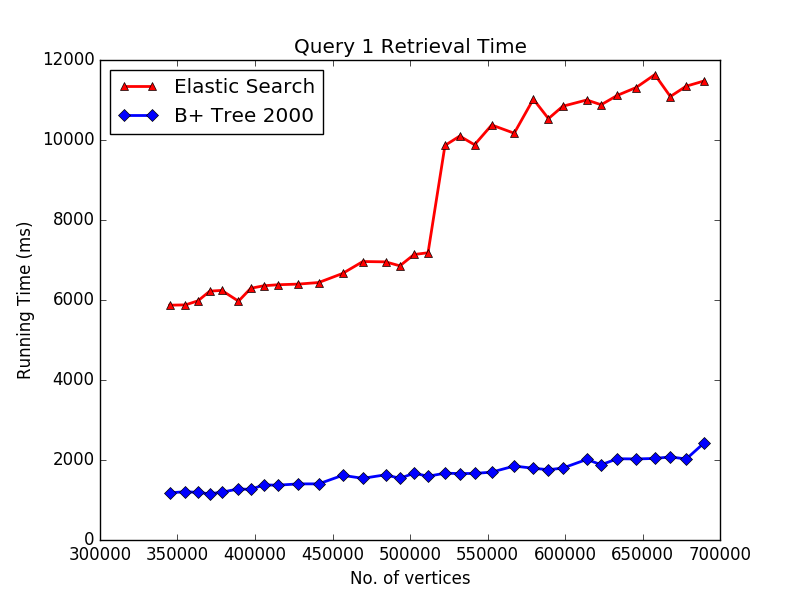
\includegraphics[width=.8\linewidth]{Figures/figure_2}
  \captionof{figure}{Vertex Retrieval Time}
  \label{fig:test1}
\end{minipage}%
\begin{minipage}{.5\textwidth}
  \centering
  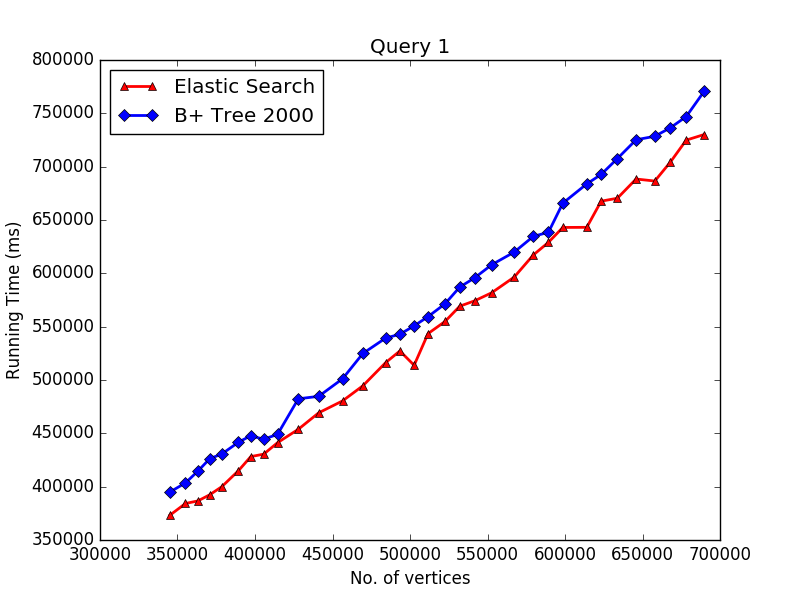
\includegraphics[width=.8\linewidth]{Figures/figure_1}
  \captionof{figure}{Query Running Time}
  \label{fig:test2}
\end{minipage}
\end{figure}
$\:$\\
From the graph we can see that though the in graph index structure out performs the elastic search index in terms of just the data retrieval (the primary task of the index), the in graph data index has somehow caused the overall query to slow down. 

\subsection{Hyperparameter: Fan-out factor}
The in graph indexed used to produce the above results is a B+ Tree with a fan out factor of 2000 (i.e. maximum no. of children of a node is 2000). This is a hyper-parameter that can be searched over to get the most optimal value. For our experiments we did not perform any hyper parameter search but instead chose an intuitive value after checking the query timings with a few values of the fan out factor. 

\section{Error analysis and optimizations}
In the above section we observed a that the query utilizing the in graph index data structure was slower than the query utilizing the elastic search index. A prominent reason behind this could be that the in the query using the in graph index data structure, there is an explicit separation of the data retrieval step and data processing step. While on the other hand the query utilizing the elastic search index might derive benefits from pipelining of the two parts of the query. (Note: Pipelining, here, refers to the general definition of pipelining popular in the DBMS community). In order to confirm this hypothesis, a simple experiment would be to separate the query utilizing the elastic search index into two parts and obtain the query timings. Shown below is the query timing graph for such a case. 

\begin{figure}[H]
\centering
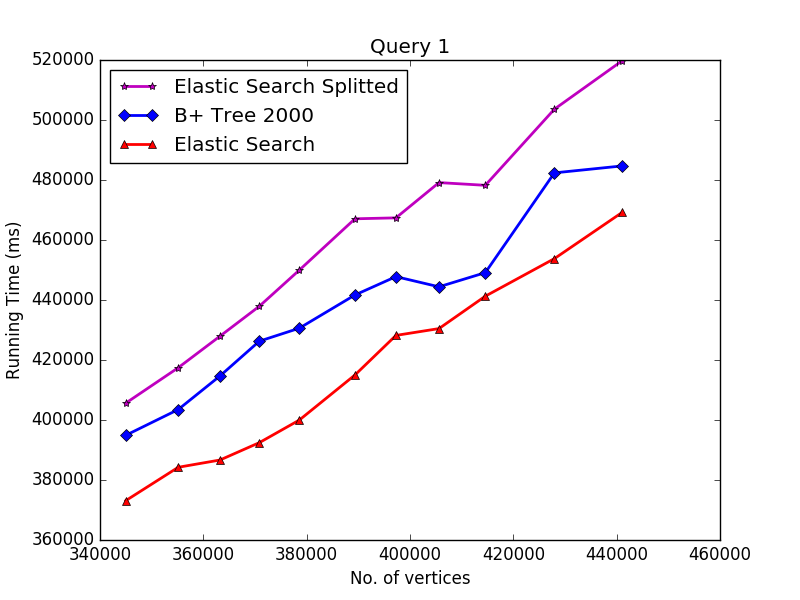
\includegraphics[width=.8\linewidth]{Figures/figure_1-100}
\captionof{figure}{Query Running Time}
\label{fig:test1}
\end{figure}
$\:$\\
While we now have some idea on what might be going wrong, how this can be rectified is still to be resolved. As an attempt to resolve this we try to combine the two parts of the query utilizing the in graph index structure into one. This can be done by traversing the index to retrieve information in a single gremlin query rather than in Java-like code and then calling the data processing steps on this traversal.  We used .repeat() and .until() steps to traverse over our in graph index data structure. The traversal that we came up with to traverse through the B+ Tree in a single gremlin query is shown below:
\\
\begin{lstlisting}
g.V().has("index_id", -1).out().has("name",indexName)           //index root
  .repeat(
    __.outE("INDEX_EDGE")
      .not(__.has("min", P.gte(dateVar)))
      .not(__.has("max", P.lte(initDateVar)))
      .inV()
  )
  .until(__.outE("INDEX_EDGE").count().is(0))
  .outE("INDEX_DATA_EDGE")
  .has("val", P.gte(initDateVar)).has("val", P.lte(dateVar)).inV()
\end{lstlisting}
$\:$\\
Combining this with the data processing step from the sample query we have been using, we get a combined query as shown below:
\\
\begin{lstlisting}
g.V().has("index_id", -1).out().has("name",indexName)
  .repeat(
    __.outE("INDEX_EDGE")
      .not(__.has("min", P.gte(dateVar)))
      .not(__.has("max", P.lte(initDateVar)))
      .inV()
  )
  .until(__.outE("INDEX_EDGE").count().is(0))
  .outE("INDEX_DATA_EDGE")
  .has("val", P.gte(initDateVar)).has("val", P.lte(dateVar)).inV()
  .group()
  .by{ it.value("po_creationDate").getYear()+1900 }
  .by(group().by(T.label).by(group().by{
    int len = it.value("length");
    if (len < 40) {
        return "short";
    } else if (len < 80) {
        return "one liner";
    } else if (len < 160) {
        return "tweet";
    } else {
        return "long";
    }}));
\end{lstlisting}
$\:$\\
The comparison of this query with the one utilizing elastic search is shown below. The elastic search index is still out performing ours in terms in the full query time. 

\begin{figure}[H]
\centering
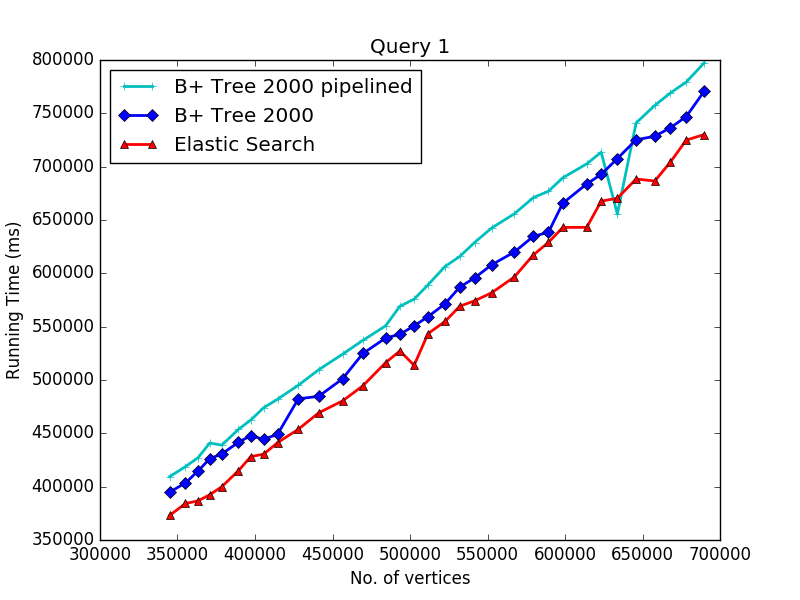
\includegraphics[width=.8\linewidth]{Figures/figure_1-200}
\captionof{figure}{Query Running Time}
\label{fig:test1}
\end{figure}
$\:$\\
Clearly we have not been able to come up with the optimal index traversal gremlin query. We experiment with a few things like if the order of the data retrieved is affecting the overall processing time but have not received any convincing results yet. One prime thing we came across was the bulk optimizations that are internal to JanusGraph. Interestingly putting an explicit barrier step after data retrieval does the greatest improvement to our timings.
\begin{figure}[H]
\centering
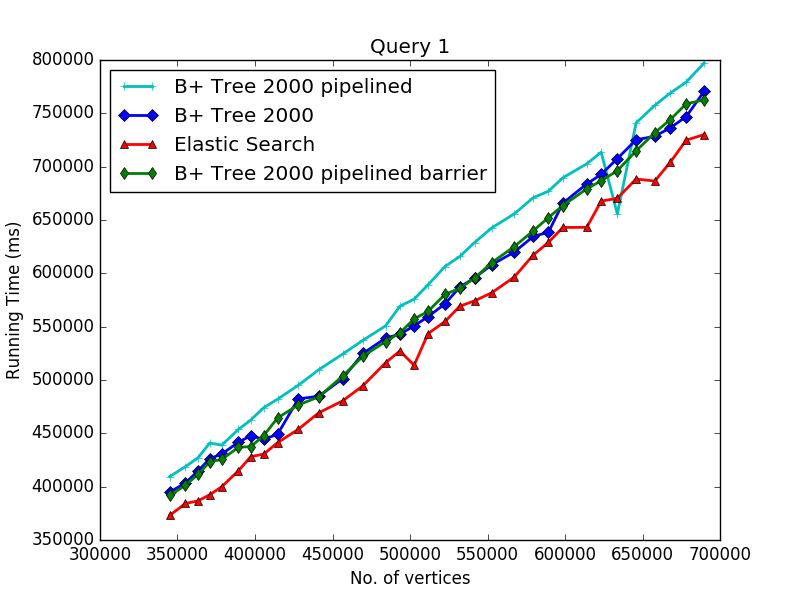
\includegraphics[width=.8\linewidth]{Figures/figure_1-300}
\captionof{figure}{Query Running Time}
\label{fig:test1}
\end{figure}
$\:$\\
In order to obtain greater insights on what was going wrong we started looking at other queries in the workload and surprisingly there were quite a few of them where the queries utilizing our index executed faster than the ones utilizing the elastic search index. This has been shown below:

\begin{figure}[H]
\centering
\begin{minipage}{0.33\textwidth}
  \centering
  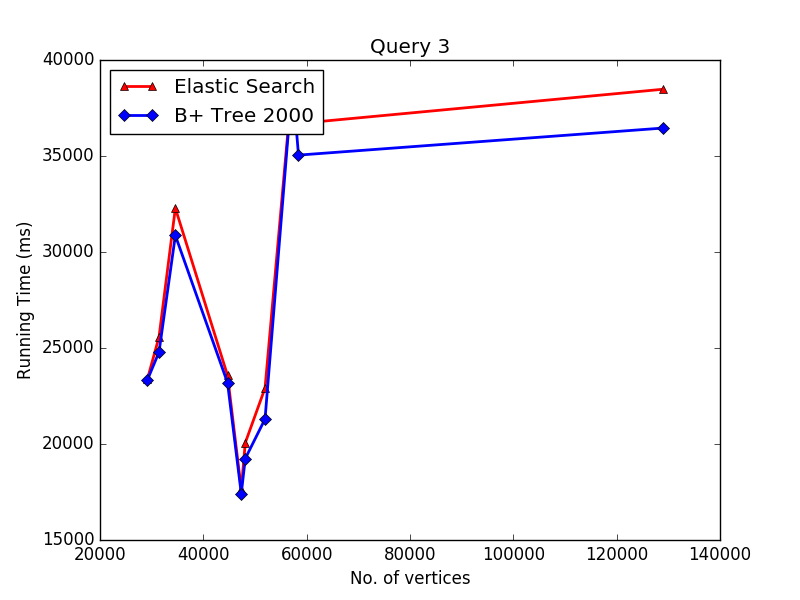
\includegraphics[width=1\linewidth]{Figures/figure_3}
  \captionof{figure}{}
  \label{fig:test1}
\end{minipage}%
\begin{minipage}{.33\textwidth}
  \centering
  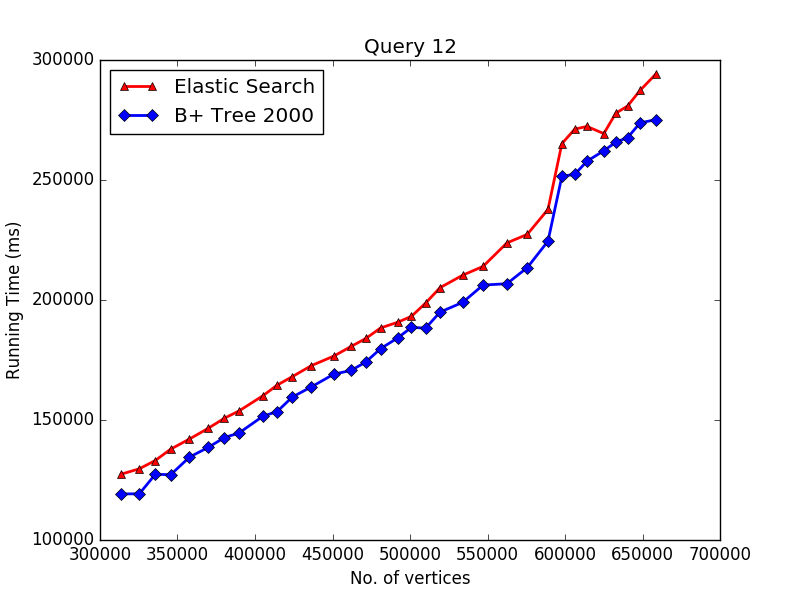
\includegraphics[width=1\linewidth]{Figures/figure_12}
  \captionof{figure}{}
  \label{fig:test2}
\end{minipage}
\begin{minipage}{.33\textwidth}
  \centering
  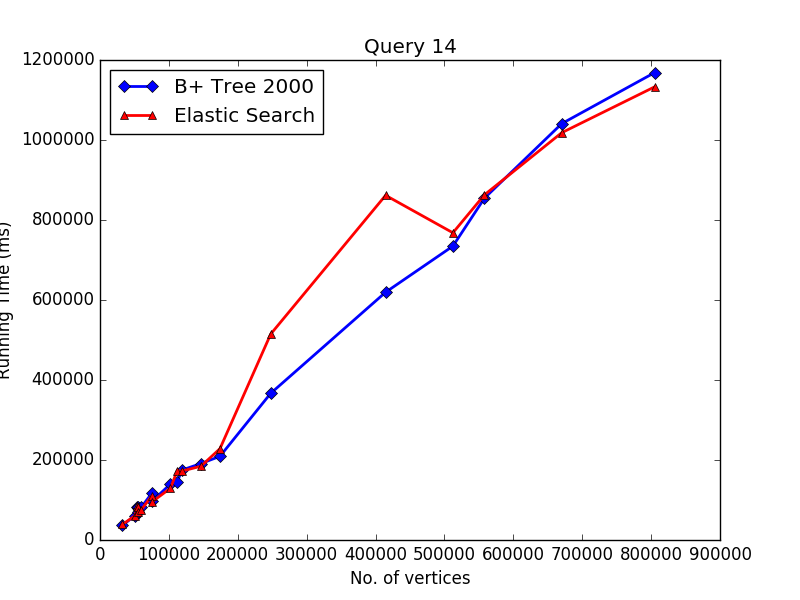
\includegraphics[width=1\linewidth]{Figures/figure_14-1}
  \captionof{figure}{}
  \label{fig:test2}
\end{minipage}
\end{figure}
$\:$\\
Why the performance in query 1 degrades is something that remains to the ascertained yet. How can we further improve the performance and make this much more faster than elastic search would be another interesting thing to explore and find out.

% \subsection{The Queries module}
% The Queries are in the codebase all inherit from the \textit{Query} class. This enforces the Query classes to have a function runQuery() that returns an object of \textit{QueryResult}. The \textit{QueryResult} object allows storage of various parameters that are useful in query runtime analysis. These are
% \begin{itemize}
% \item Count of vertices returned
% \item Time to run query
% \item Time to traverse index
% \item The result returned
% \end{itemize}




\section{Results}

\paragraph{The result sheet}
$\:$\\
The aforementioned Google Sheet \cite{runtime} contains all the experimental results we have obtained. The sheets \textit{[Final] Query Running Time} and \textit{[Final] Vertex Retrieval Time} contain our final query timings when we ran them on Aryabhata on the 1GB dataset. We have the timings for queries 1, 3, 10, 12 and 14. These are the queries that used our B+ Tree index on \textit{po\_creationDate} property.

\section{Brief description of the code repository}

\paragraph{PerformanceTester}
$\:$\\
\textit{PerformanceTester} is a class created to aid the running of queries to get reliable experimental data of run times. This class runs the queries in the Queries folder. These queries are expected to inherit from the \textit{Query} class. The \textit{PerformanceTester} takes the class name of query to run, the parameter file index in \textit{substitution\_parameter} folder, the number of lines to skip in the parameter file and the \textit{conf} file to use to make connection to the JanusGraph DB.
\\\\
Running the \textit{PerformanceTester} runs the specified query using the specified parameter file. It generates a .txt file that has various metrics like the average, median and standard deviation of the query run times and the index traversal times. This .txt file is generated in a \textit{query\_results} folder.


\paragraph{Using the Performance Tester class}
$\:$\\
Create the jar of the java module. The usage for running the jar is
\\\\
\textit{java -cp Utilities-1.0-SNAPSHOT-jar-with-dependencies.jar main.PerformanceTester\\<queryClassName(only the endclassname)> <param\_number> <skiplines> [<confFile>]}
\\\\
Example:
\\
\textit{java -cp Utilities-1.0-SNAPSHOT-jar-with-dependencies.jar main.PerformanceTester BPIndexQuery1\_1 1 1 local}
\\\\
The \textit{query\_results}, \textit{substitution\_parameter} and \textit{conf} folder will need to be present along with the jar when it is run. Sample of these can be obtained from our git repository \cite{repo}.
\\\\
The times we obtained by running queries can be accessed at result spreadsheet\cite{runtime}




% Chapter Template

% Chapter Template

\chapter{Query Rewrite Framework} % Main chapter title

\label{Chapter 6} % Change X to a consecutive number; for referencing this chapter elsewhere, use \ref{ChapterX}

So far, we have seen that we are dependent on including Index tree traversal in the query. To compete with Elastic Search indexes, we must be able to seamlessly use our indexes in general gremlin queries. This creates the need to be able to automatically rewrite a gremlin query with index tree code so that we have a true proof of concept of the applicability of our indexes.

\paragraph{Methodology}
$\:$\\
Our first task in the rewriting procedure is to identify part of the gremlin  query to be rewritten. For this, we break to query into a list of \textit{Traversal Steps} using the \textit{GremlinGroovyScriptingEngine}. We then look for \textit{HasStep} which lie immediately after some \textit{GraphStep} which have all vertices in the Graph. The key attribute of this \textit{HasStep} is identified. We then check whether there exists an index applicable for our given attribute. We thus need the metadata of the indexes. Here come handy the edges from the super-index to the index roots which have properies representing the metadata.
\\\\
Just looking at the first HasStep is not much meaningful. We should consider all consecutive HasSteps after the GraphStep for applying the index. To achieve this, we keep looking at the key attribute in all HasSteps till we find one on which we can use our index. After this, in the next consecutive \textit{.has()}, we only look for the presence of the same key attribute. All these HasStep collectively define a range of values within which the key attribute should be in the vertices of the result. We maitain 2 variables: $minVal$ and $maxVal$. Initiall these values are set to the extremes of the datatype of the key (so as to return all possible values i.e. full range). Every HasStep on the key shrinks this range. Finally, the output query has the GraphStep followed by the index traversal code for the range $[minVal, maxVal$] on the key attribute and the other HasSteps in the consecutive HasStep list and any other gremlin steps which may follow this list.
% Chapter Template

% Chapter Template

\chapter{Conclusion} % Main chapter title

\label{Chapter 7} % Change X to a consecutive number; for referencing this chapter elsewhere, use \ref{ChapterX}

In this chapter we briefly summarize our contributions and put forth several possible future directions for the project that the further extensions might be based on.

\section{Key Contributions}
A key contribution of our work is that it serves as a proof-of-concept showing that in database index structures can be as efficient as the state of the art elastic search indexes. This also in some sense offers a better stability of the complete system by reducing a moving component of a third party application and thus reducing a large number of places where frequent faults or crashes can occur. Not only stability, this concept also offers a very vast flexibility to the user in terms of the design of index structure, which was previously restricted to what is available in elastic search or any other third party indexing application.\\
\\
With the introduction of rewrite engine we can now in fact take a simple user gremlin query and optimize it ourselves to use the in database/graph index structures if available, which also makes our index structures equally easy to use like any other indexing mechanism like elastic search or solr. This work also opens up a much larger new area for any audience willing to try a new innovative index structure and they will be only restricted by the fact that their index must be representable as a graph. We already support the pre-implemented versions of B-Tree and B+ Tree index structures for the aforementioned infrastructure which are one of the most common index structures in the databases community.

\section{Further Extensions}
This section describes in brief some of the several possible future directions directions of this work.

\paragraph{Selecting amongst multiple available indexes}
$\:$\\
We currently select the first possible usage of index to rewrite the given query. But, suppose there are many indexes with different parameters on same key, how to select one? An improvement over this would be to add a metric for selecting the best index amongst a variety on indexes available on different attributes of a gremlin query. 

\paragraph{Extending to other databases}
$\:$\\
Also, this work is clearly not restricted to a single graph database but applies to a large variety of them. Extension implementations of the same for other Graph DBs like Neo4J is likely to generalize these kind of indexes even further. Converting the system into a easy to use plugin for Janusgraph/Neo4J is a direct way popularizing this kind of index in the community.

\paragraph{Adding more index structures or a GiST}
$\:$\\
Expanding this work into something where any user can be allowed to just add code to a few functions to introduce another kind of new/novel index can greatly accelerate the usage of this kind of index structures. Another possible way to add the power of a generalized search index would be to implement something like the GiST (Generalized Search Tree) mentioned by Hellerstein et. al \cite{GiST}.

\paragraph{Other kinds of traversals}
$\:$\\
Storing index structures along with the data opens multiple new avenues which can be exploited to optimize the execution of queries on Graph DBs. Apart from the traditional index-to-data traversal, data-to-index and index-to-index movements too are possible now.

\subparagraph{Data to Index}
$\:$\\
Moving from Data to Index can help us easily determine the key on which the index is based given the data vertex. This might at first not seem to be really useful owing to the fact that if the indexing key is already a property of the vertex, then once we have the vertex, we can directly find its value instead of going to the index vertex and adding one extra vertex fetch.\\
\\
However, consider the case where the index is present on the some aggregation of keys rather than directly the key. For example an index on the percentile of marks received by a student can help to trivially compute his percentile which in the absence of such an index would involve multiple vertex fetches.

\subparagraph{Index to Index}
$\:$\\
Another possible extension to this is the \textbf{Index-to-Data-to-Index} traversal which can help us answer queries like what percentile of salary is being received by the students with top x percentile marks.\\
\\
In this kind of queries, an execution can be framed that using the index structures, filters the data swiftly to get to a specific set of vertices/data nodes. This execution can then use the idea from the data to index traversal to answer the aggregation queries on this filtered set of nodes.\\
\\
Creating/obtaining a set of workloads / benchmark specifically to observe the effects of these kind of optimizations (and novel use of index structures) is an issue one might have address before jumping right into these kinds of executions/traversal though.

\paragraph{Creation of  index structures automatically based on workload}
$\:$\\
Analysis of workload of a set of queries can help in further refining the indexing in Graph DBs. We can suggest suitable indexes to be created internally without the knowledge of the user and use these indexes to automatically modify the queries for making use of these indexes. Apart from simple suggestion of indexes based on workloads, this requires analysis of each index to judge whether it offers a good trade-off in terms of performance improvement over increase in size of the graph (due to the additional vertices and edges we add to accommodate the index structure).
% % Chapter Template

% Chapter Template

\chapter{Query Rewrite Framework} % Main chapter title

\label{Chapter 6} % Change X to a consecutive number; for referencing this chapter elsewhere, use \ref{ChapterX}

So far, we have seen that we are dependent on including Index tree traversal in the query. To compete with Elastic Search indexes, we must be able to seamlessly use our indexes in general gremlin queries. This creates the need to be able to automatically rewrite a gremlin query with index tree code so that we have a true proof of concept of the applicability of our indexes.

\paragraph{Methodology}
$\:$\\
Our first task in the rewriting procedure is to identify part of the gremlin  query to be rewritten. For this, we break to query into a list of \textit{Traversal Steps} using the \textit{GremlinGroovyScriptingEngine}. We then look for \textit{HasStep} which lie immediately after some \textit{GraphStep} which have all vertices in the Graph. The key attribute of this \textit{HasStep} is identified. We then check whether there exists an index applicable for our given attribute. We thus need the metadata of the indexes. Here come handy the edges from the super-index to the index roots which have properies representing the metadata.
\\\\
Just looking at the first HasStep is not much meaningful. We should consider all consecutive HasSteps after the GraphStep for applying the index. To achieve this, we keep looking at the key attribute in all HasSteps till we find one on which we can use our index. After this, in the next consecutive \textit{.has()}, we only look for the presence of the same key attribute. All these HasStep collectively define a range of values within which the key attribute should be in the vertices of the result. We maitain 2 variables: $minVal$ and $maxVal$. Initiall these values are set to the extremes of the datatype of the key (so as to return all possible values i.e. full range). Every HasStep on the key shrinks this range. Finally, the output query has the GraphStep followed by the index traversal code for the range $[minVal, maxVal$] on the key attribute and the other HasSteps in the consecutive HasStep list and any other gremlin steps which may follow this list.

%-----------------------------------------------------------------------------
%	THESIS CONTENT - APPENDICES
%-----------------------------------------------------------------------------

\appendix % Cue to tell LaTeX that the following "chapters" are Appendices

% Include the appendices of the thesis as separate files from the Appendices folder
% Uncomment the lines as you write the Appendices

% % Appendix A

% \chapter{How to run the Project} % Main appendix title

% \label{AppendixA} % For referencing this appendix elsewhere, use \ref{AppendixA}

% \section{Choice of Database}
% We essentially deal with Graph databases for the purpose of creating index and running benchmark queries on it. We use JanusGraph //todo with Cassandra //todo DB as the storage backend and Elastic Search //todo as the indexing backend. The choice of Cassandra was based on the need for frequent writes as a part of testing, which is primarily what cassandra is optimized for. The indexing backend is used to directly compare the query timings using our in Graph index structure to the timings obtained using elastic search index. JanusGraph by deafult, uses Gremlin (from Apache Tinkerpop3 //todo ) as its query interface. JanusGraph is also an open source, community developed project. We also found that it to behaving a larger and fast growing community support and adoption.

% \section{Getting up and running with the code base}

% Please check the wiki from the github-repository which should have detailed instructions on how to get started with the setup of the java codebase. Access to the repository can be requested from our Advisor to the project.

% \section{Loading Data}
% \section{Build the (Ghost) Index Structure}
% \section{Running queries from the codebase}
% \section{Using the query rewrite framework}

%\include{Appendices/AppendixB}
%\include{Appendices/AppendixC}

%-----------------------------------------------------------------------------
%	BIBLIOGRAPHY
%-----------------------------------------------------------------------------

%\printbibliography[heading=bibintoc]

%-----------------------------------------------------------------------------


\begin{thebibliography}{99}

\bibitem{benchmark} Benchmark: http://ldbcouncil.org/developer/snb
\bibitem{ldbcQueries} SNB Queries Specifications: http://ldbc.github.io/ldbc\_snb\_docs/ldbc-snb-specification.pdf
\bibitem{datagen} LDBC Data Generator: https://github.com/ldbc/ldbc\_snb\_datagen
\bibitem{gremlin} Gremlin reference book: http://kelvinlawrence.net/book/Gremlin-Graph-Guide.html
\bibitem{tinkerpop1} Tinkerpop Documentation: http://tinkerpop.apache.org/docs/current/reference/
\bibitem{tinkerpop2} Tinkerpop Java Documentation: http://tinkerpop.apache.org/javadocs/current/core/
\bibitem{book1} Towards Integrated Graph Algebra for Graph Pattern Matching with Gremlin: Harsh et al
\bibitem{book2} The Gremlin Graph Traversal Machine and Language: Marko A. Rodriguez
\bibitem{runtime} Query run times: https://docs.google.com/spreadsheets/d/1lSBP4IWh5VKFXzT6
\\
qyYzQJn\_R93dUtRdPldVc9AqR38/
\bibitem{repo} Git Repository: https://github.com/Prakhar0409/Ghost-Index-in-Graph-DB
\bibitem{GiST} Generalized Search Tree: http://db.cs.berkeley.edu/papers/vldb95-gist.pdf


\end{thebibliography}


\end{document}  
